Soit $F=\{f_0,\ldots,f_n,\ldots\}$ un ensemble de \titre{symboles de fonctions} (prenant un certain nombre d'\titre{arguments}, pas le même nombre pour chaque fonction). \\

Soit $\varphi\ffonc{F}{\N}$ qui à une fonction associe le \titre{nombre d'arguments} qu'elle prend (aussi appelé \titre{arité} de la fonction)\\

\par
\titre{$F_n=\{f\in F \tq \varphi(f)=n\}$} ($F_0 =$ les constantes (on peut donc les utiliser comme arguments des autres fonctions). \\

\par
\titre{Termes} sur $F$ : On définit $T$ inductivement : \\
$\left\{ \begin{array}{l}
	(B) : F_0 \subset T \\
	(I) : \forall t_1,\ldots,t_n\in T, f\in F_n, f(t_1,\ldots,t_n)\in T
\end{array} \right.$

\titre{Lien avec les arbres ordonnés étiquetés par $F$}\\
$F=\{0,1,f,g\}\; F_0=\{0,1\}] \; F_1=\{g\} \; F_2=\{f\}$ \\
Donnons une liste (non exhaustive!) d'éléments de $T$ : \\
$0 \; ; \; 1 \; ; \; g(0) \; ; \; g(1) \; ; \; f(0,1) \; ; \; f(1,0) \; ; \; f(0,g(f(0,1))) \ldots$\\
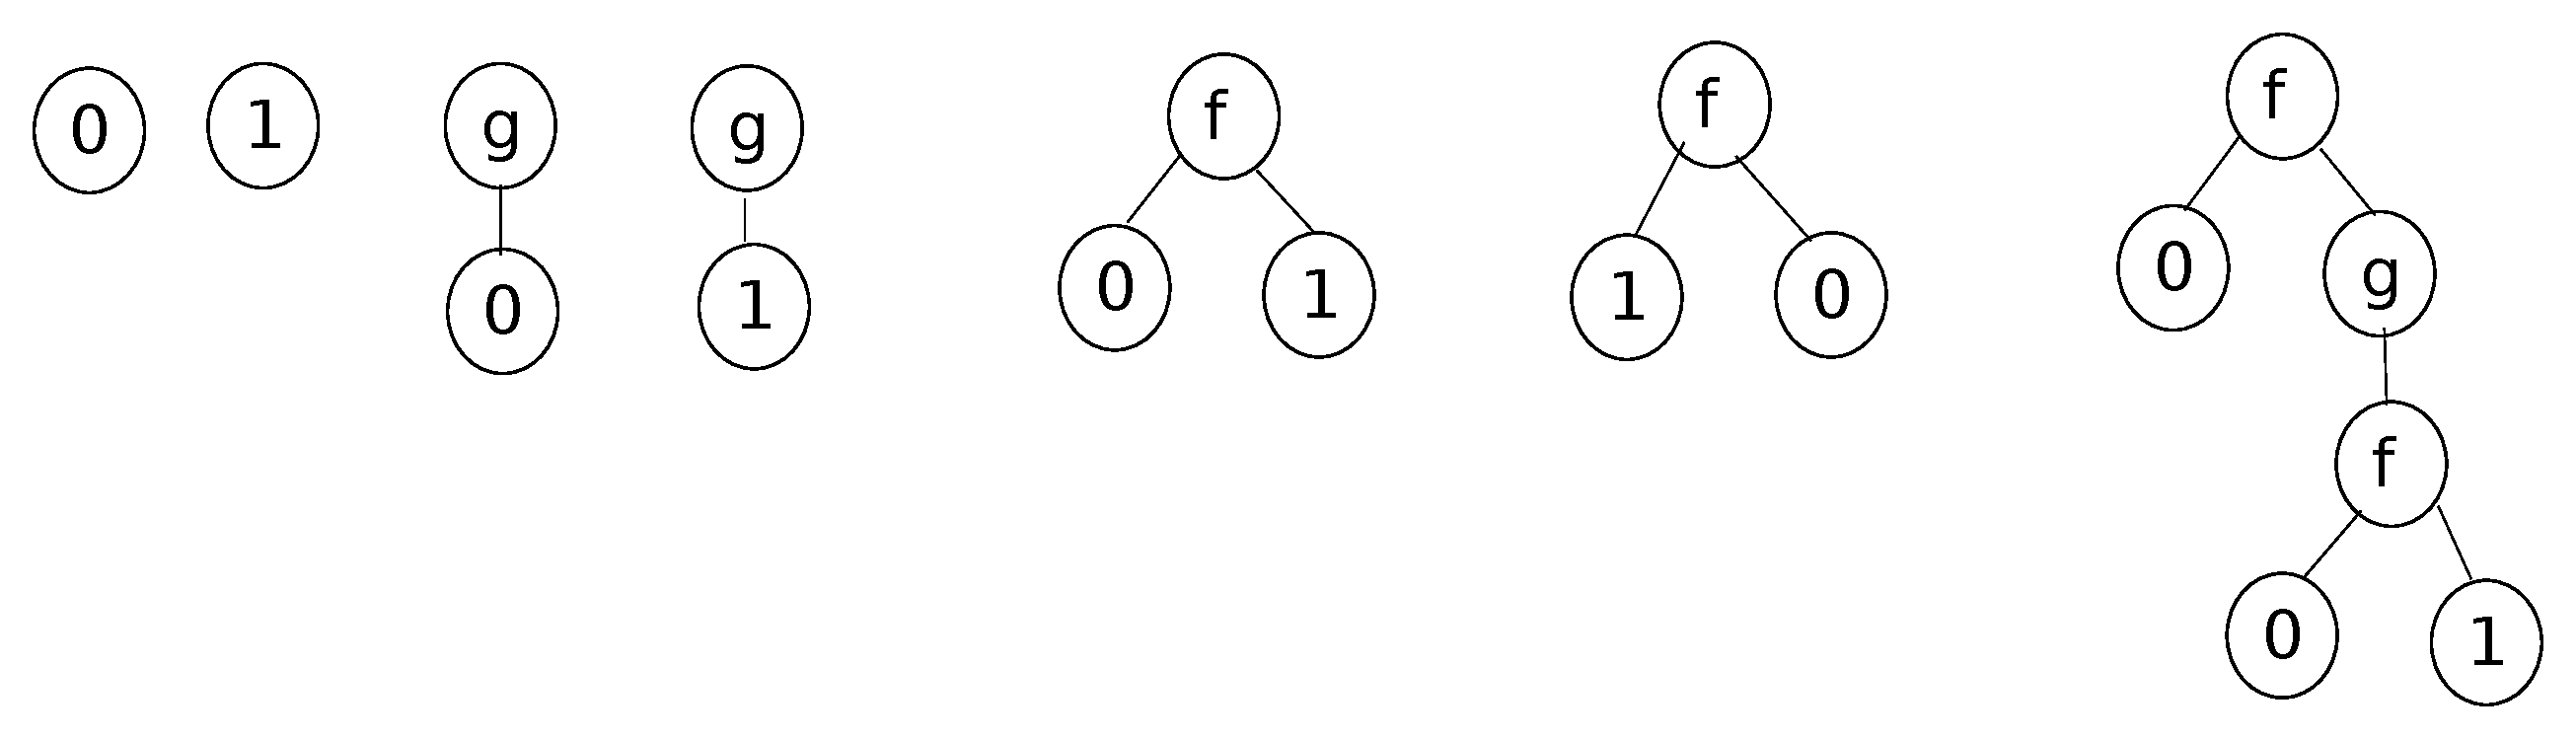
\includegraphics[width=0.8\linewidth]{D7_1.pdf}
